
\section{V - MNIST}
\begin{frame}{V - Reconnaissance d'image}
\begin{block}{Problématique}
On possède une base de données, d'image de chiffres écrit à la main. Ces images sont toutes de taille $28 \times 28$ pixels en noir et blanc. \\
La base de données est divisées en 60000 images pour l'entrainement, et 10000 autres pour la vérification.
\end{block}
\begin{figure}
	\centering
    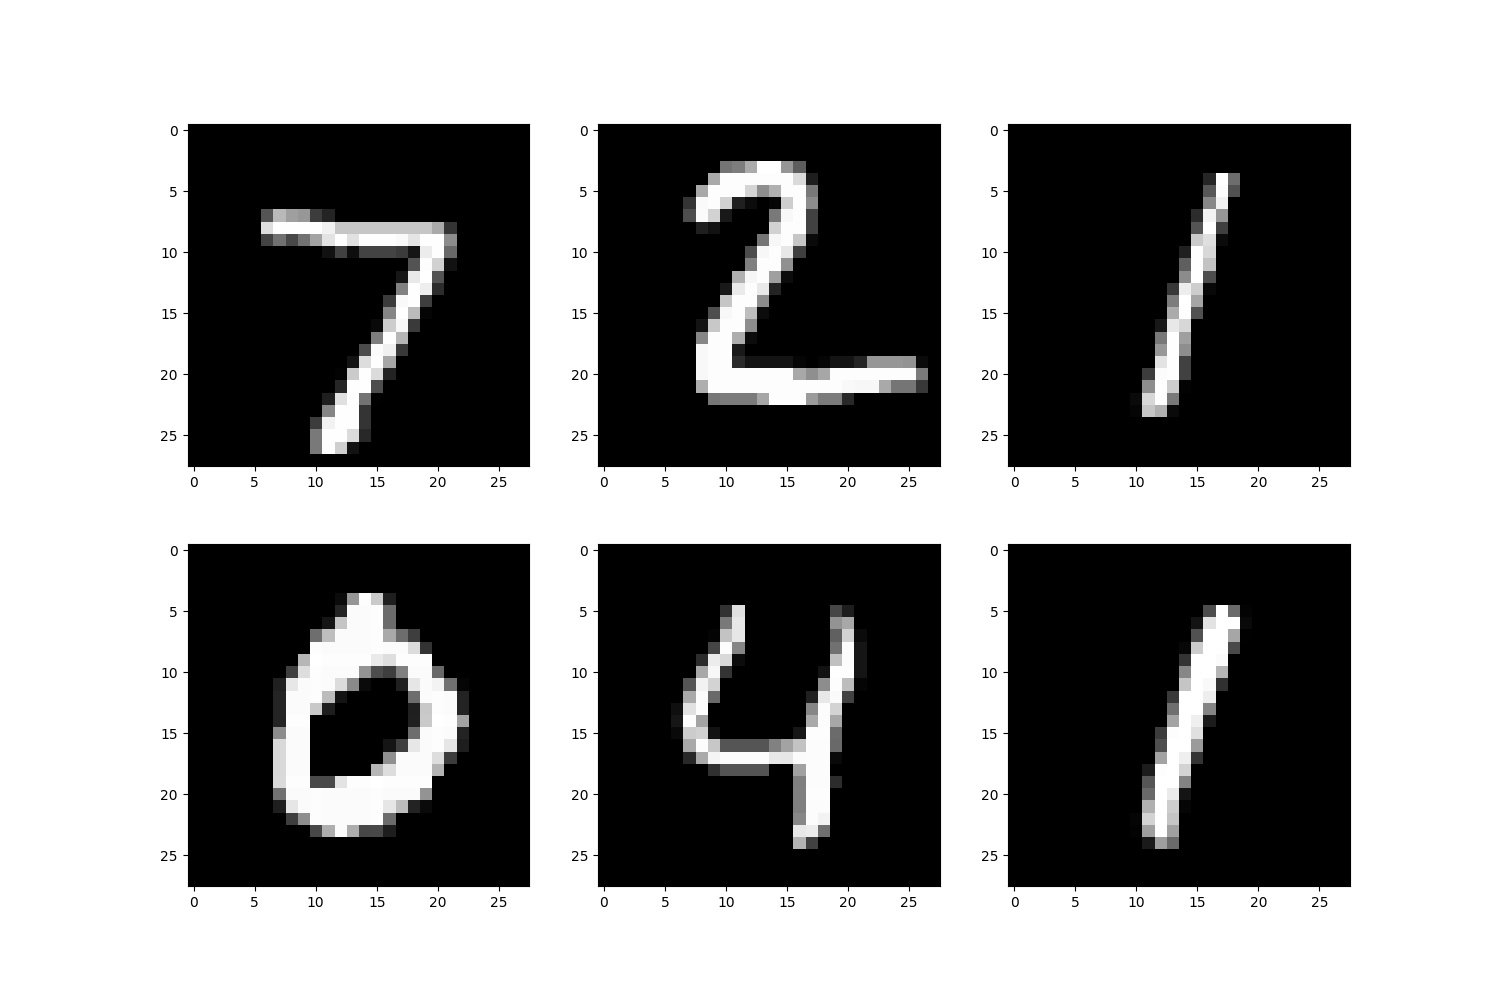
\includegraphics[width=150px]{1-mnist.jpg}
	\caption{Exemple d'images}
\end{figure}
\end{frame}

\begin{frame}{V - Apprentissage d'un problème de classification}
On prend un réseau de neurones avec $28 \times 28 = 784$ entrées, et 10 sorties. \\
\begin{block}{Softmax et Cross-entropy}
Lorsque l'on fait face à un problème de classification, il faut adapter le réseau de neurone. \\
La fonction d'activation softmax est utilisé pour la dernière couche de neurones, elle permet de normaliser les probabilités de sorties. \\
• $p_i = \frac{exp(a_i)}{\sum_{k=1}^{n}exp(e_k)}$ la probabilité de la sortie $a_i$ \\
• $\dfrac{\partial p_i}{\partial a_j} = p_i(\delta_{ij}-p_j)$ \\
La fonction de coût associée est $Cross-entropy$. \\
• $L = -\sum_{k=1}^{n}y_ilog(p_i)$ avec $y_i$ la sortie attendue \\
• $\dfrac{\partial L}{\partial a_i} = p_i - y_i$
\end{block}
\end{frame}

\begin{frame}{V - Softmax}
\begin{figure}
	\centering
    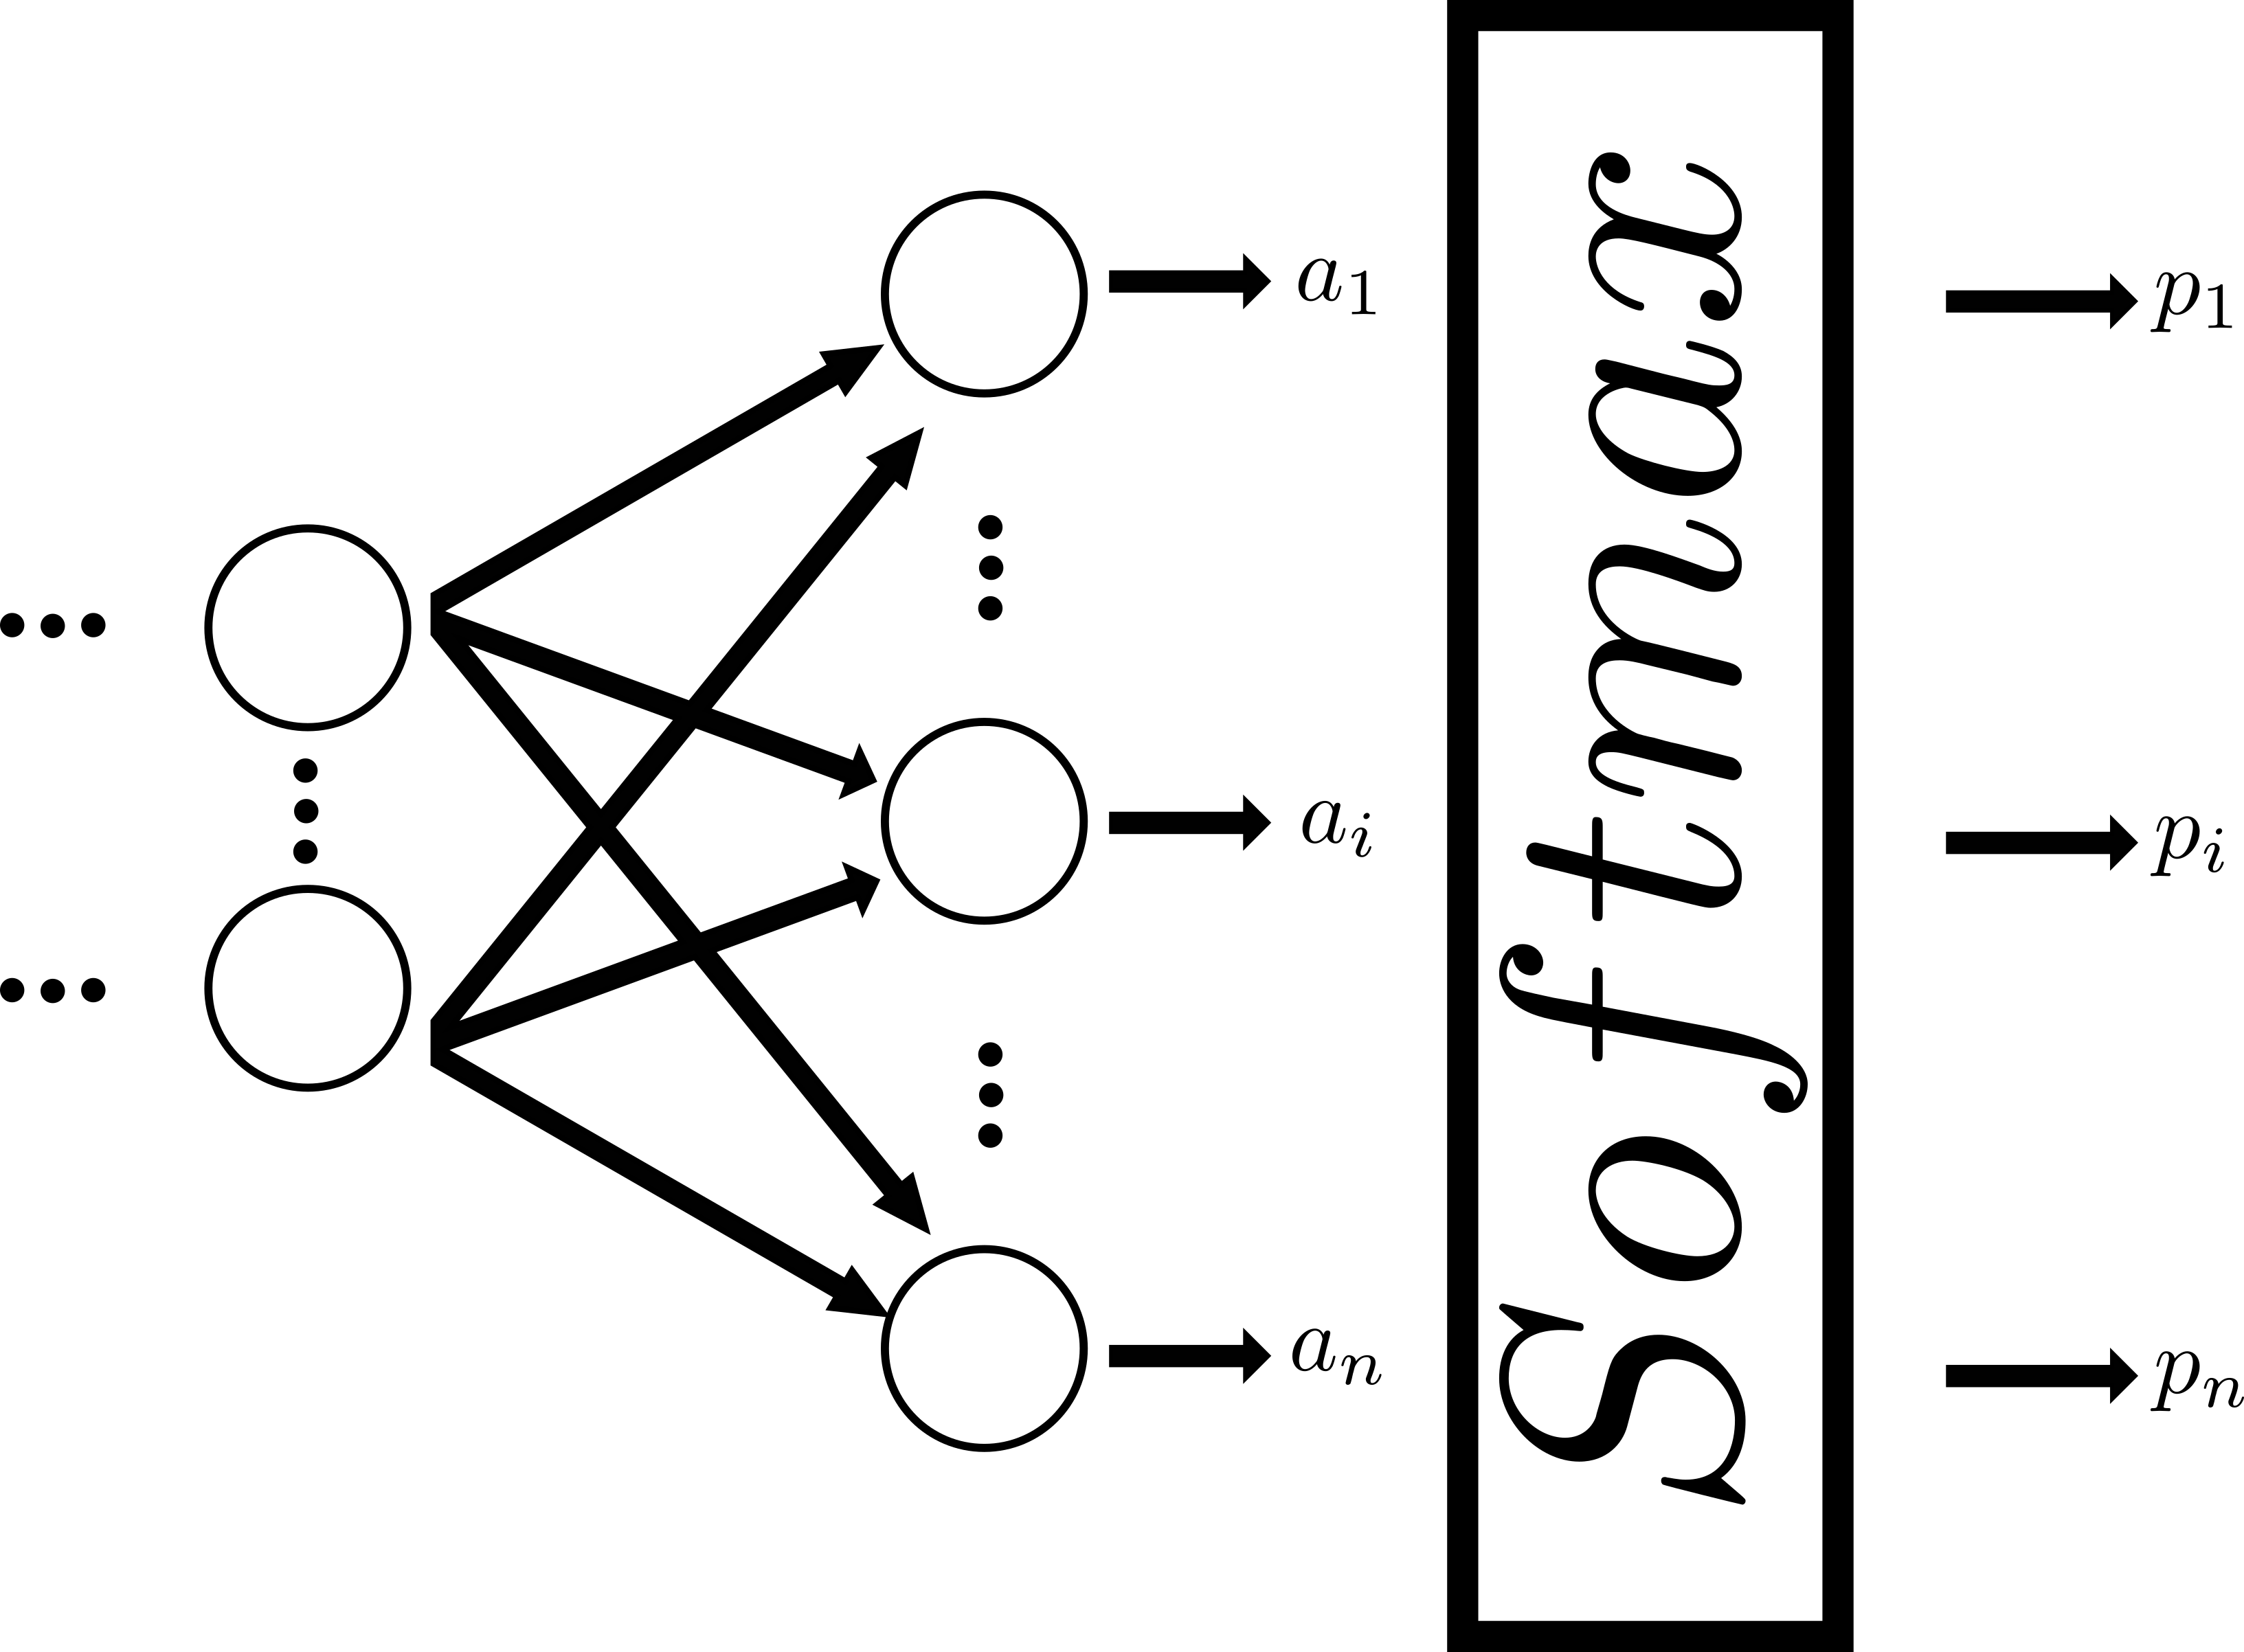
\includegraphics[height=150px]{2-Softmax.png}
	\caption{Schéma d'utilisation du Softmax}
\end{figure}
\end{frame}

\begin{frame}{V - Résultats}
Au terme de 100 générations d'entrainement, on tend à avoir 91.5\% de bonnes réponses sur les données d'entrainement et 91.3\% sur les données de validation. \\
On peut remarquer que dès le début, on à un taux de précision d'environ 10\%, c'est dû au fait que c'est un problème de classification à 10 sorties.
\begin{figure}
	\centering
    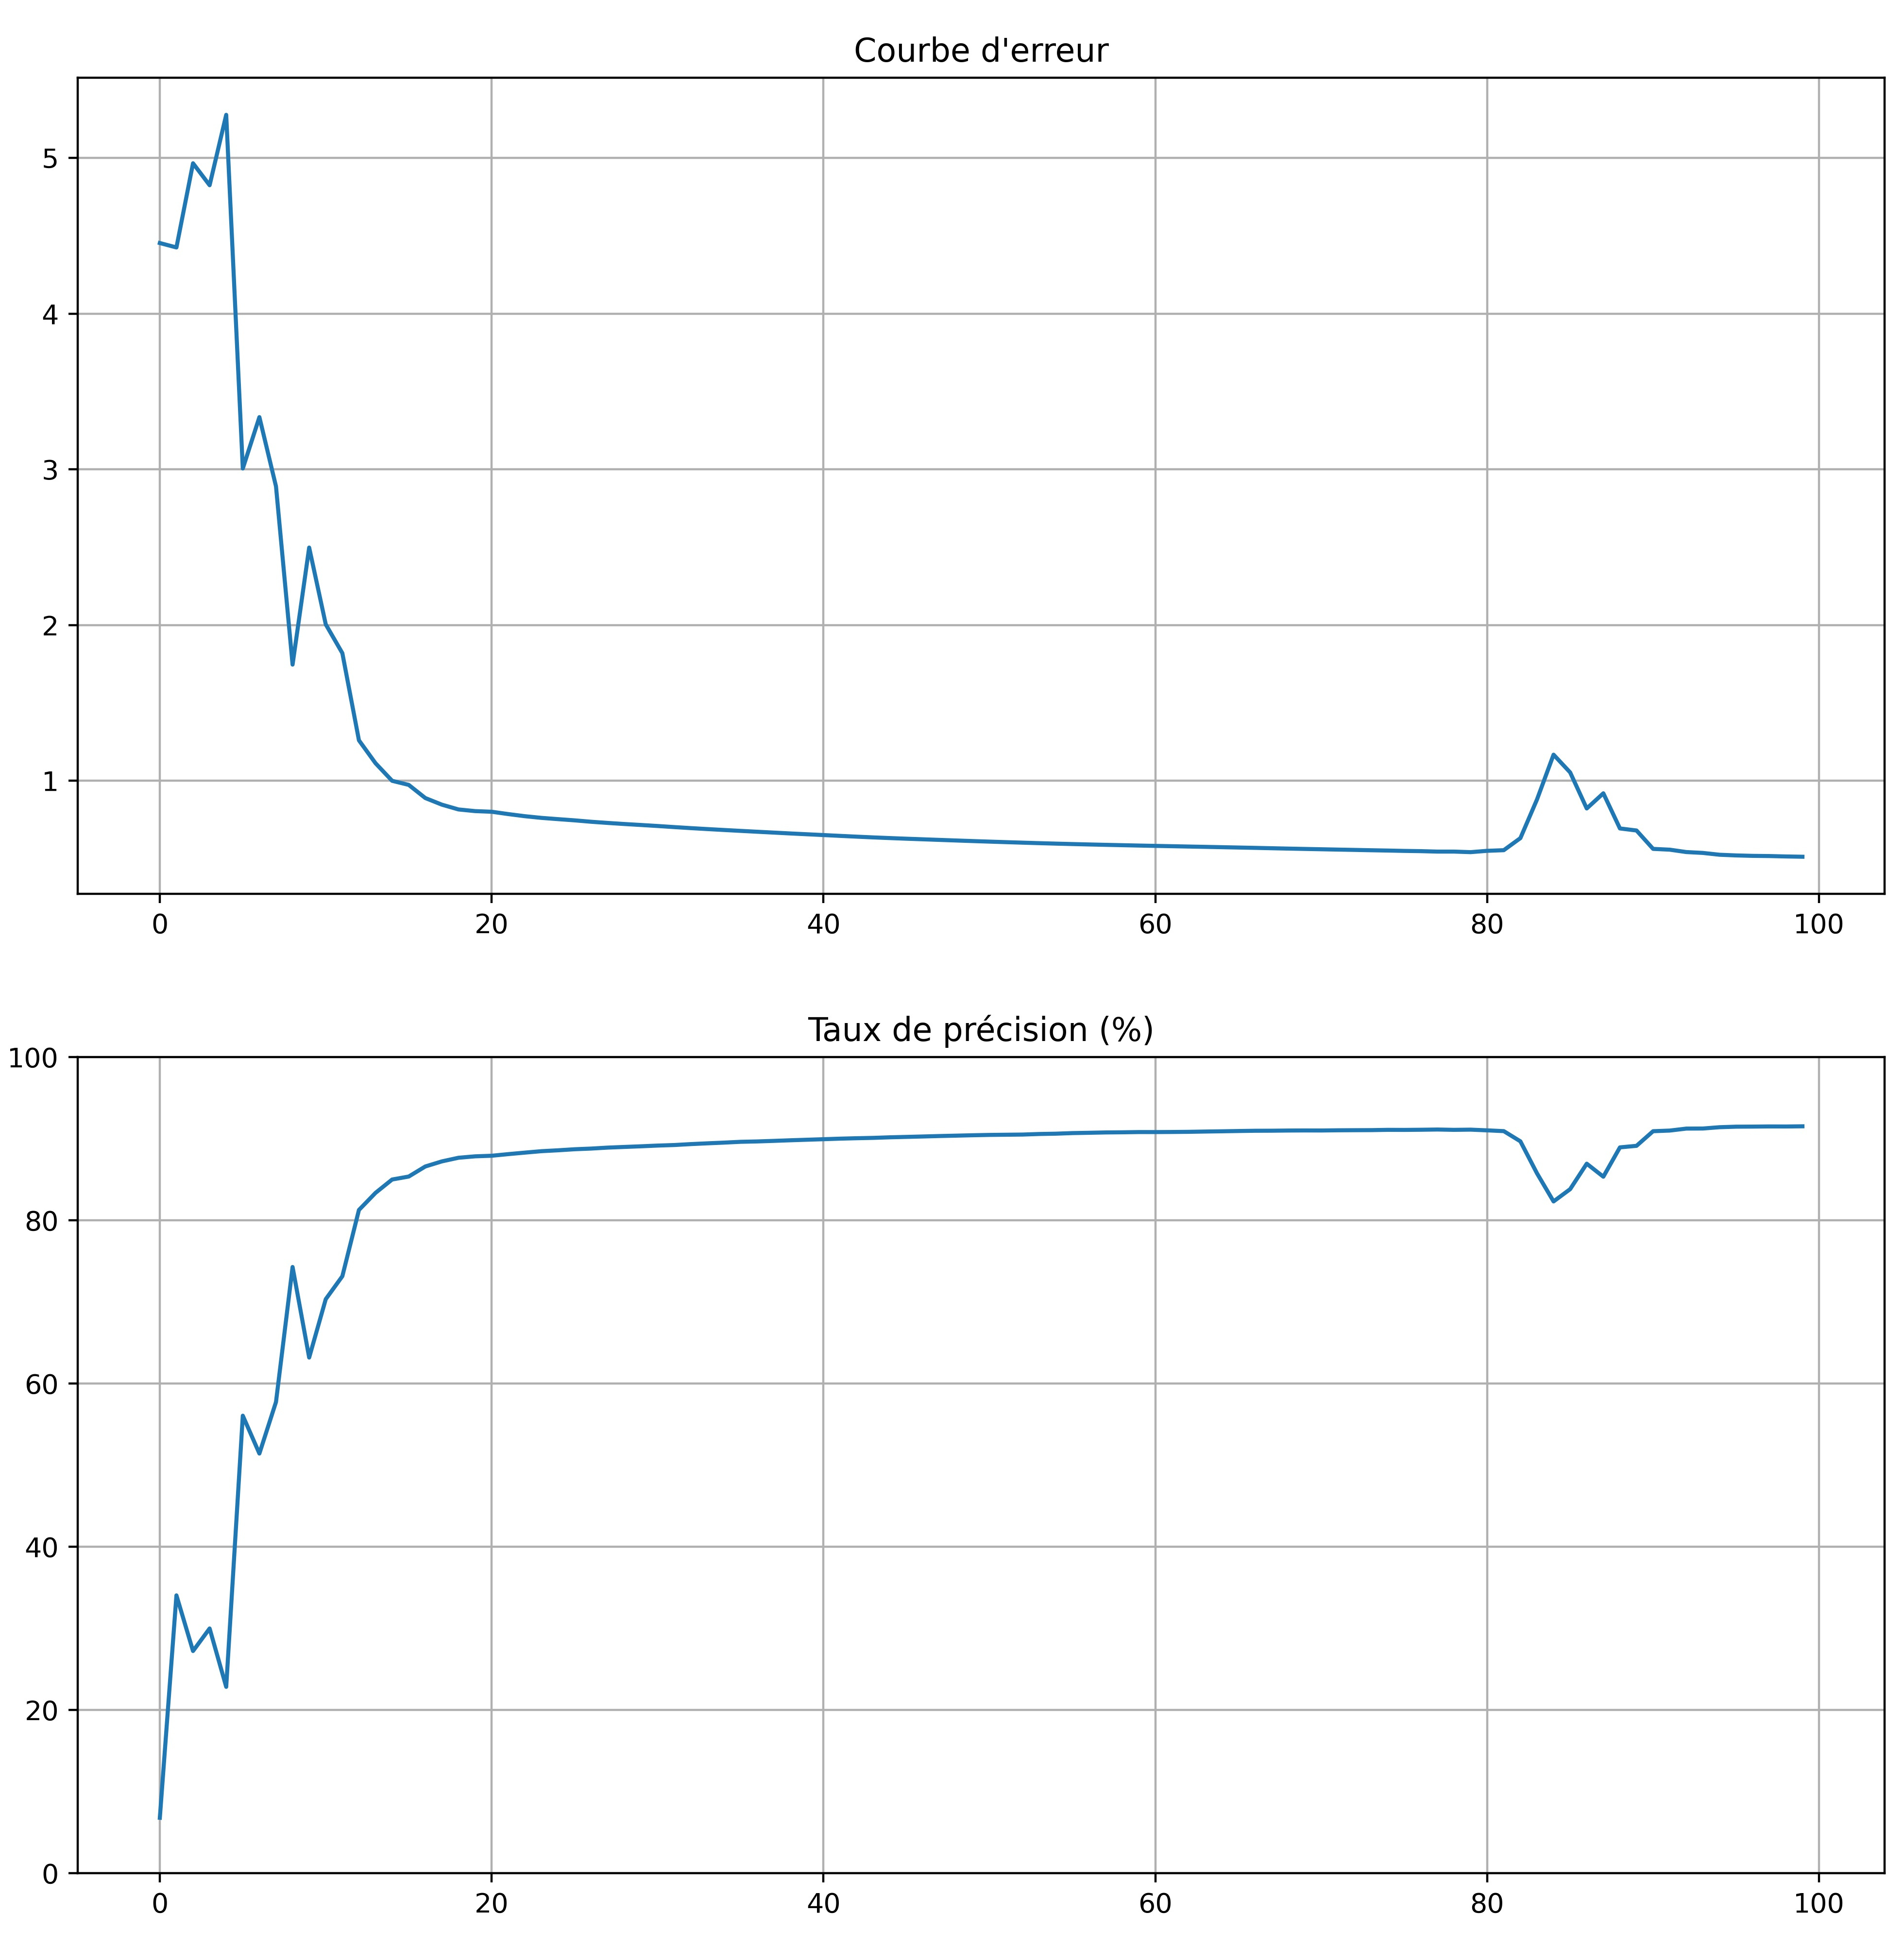
\includegraphics[height=150px]{3-Apprentissage.jpg}
	\caption{Courbes d'apprentissage}
\end{figure}
\end{frame}

\begin{frame}{V - Résultats}
\begin{figure}
	\centering
    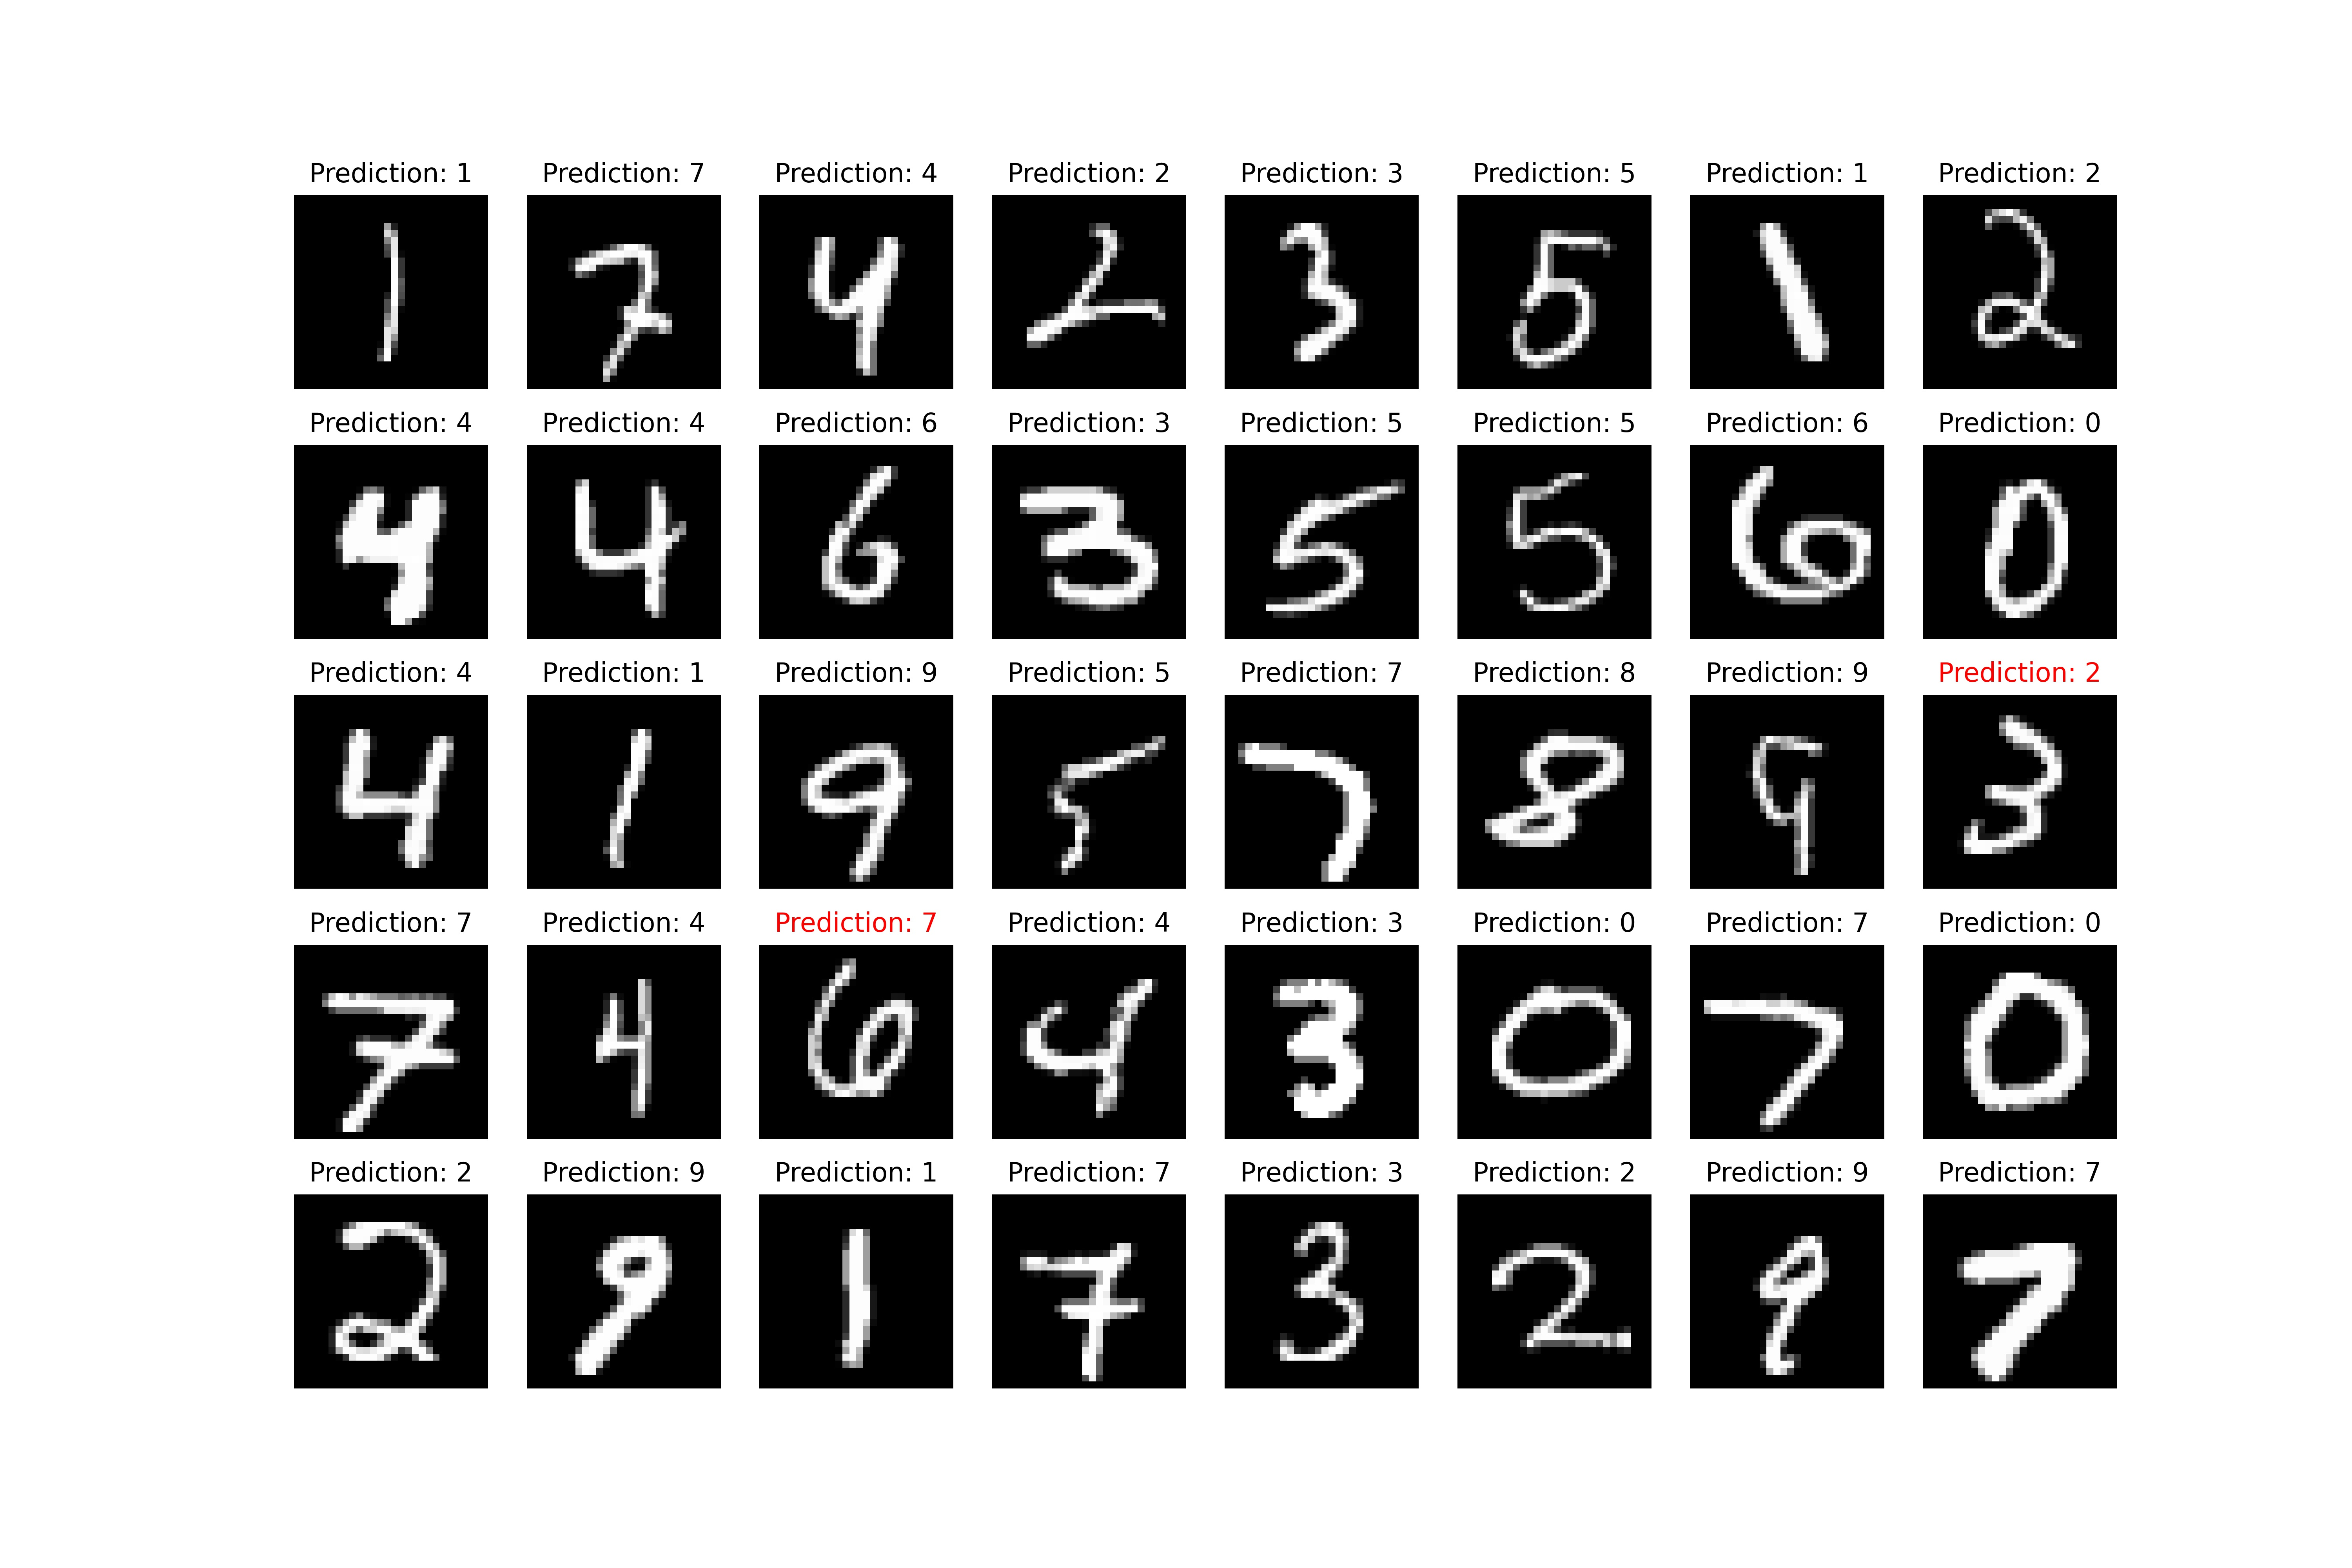
\includegraphics[height=200px]{4-Resultat.jpg}
	\caption{Exemple sur un échantillon de 40 images de validation}
\end{figure}
\end{frame}